\documentclass[tikz,margin=3mm]{standalone}
\usepackage{siunitx}
\usetikzlibrary{decorations.markings,calc}
\tikzset{
    resistor/.style={
        postaction=decorate,
        decoration={
            markings,
            mark=at position 0.5 with {
            \begin{scope}[scale=2]
                \fill[white] (-7pt,1pt) rectangle (7pt,-1pt);
                \draw (-7pt,0) -- (-6pt,0) -- (-5pt,2pt) -- (-3pt,-2pt) -- (-1pt,2pt) -- (1pt,-2pt) -- (3pt,2pt) -- (5pt,-2pt) -- (6pt,0) -- (7pt,0);
                \coordinate (x) at (-6pt,0);
                \coordinate (y) at (0,0);
            \end{scope}
            }
        }
    },
    ->-/.style={
        postaction=decorate,
        decoration={
            markings,
            mark=at position #1 with {\arrow{>}}
        }
    },
    ->-/.default=0.5
}
\begin{document}
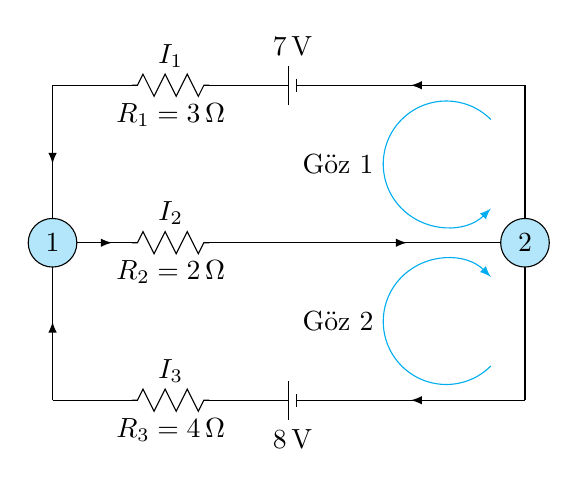
\begin{tikzpicture}[>=latex]
\draw[resistor] (0,0) -- (3,0);
\draw[->-=0.7] (0,0) -- (x);
\path (y) node[above=3pt] {$I_2$} node[below=3pt] {$R_2=\SI{2}{\ohm}$};
\draw[->-] (3,0) -- (6,0);
\draw (6,-2) -- (6,2);
\draw[->-] (6,2) -- (3.1,2);
\draw (3,2.25) -- (3,1.75) (3.1,2.08) -- (3.1,1.92) (3.05,2) node[above=0.25cm] {\SI{7}{\volt}};
\draw[resistor] (3,2) -- (0,2);
\path (y) node[above=3pt] {$I_1$} node[below=3pt] {$R_1=\SI{3}{\ohm}$};
\draw[->-] (0,2) -- (0,0);
\draw[->-] (0,-2) -- (0,0);
\draw[resistor] (0,-2) -- (3,-2);
\path (y) node[above=3pt] {$I_3$} node[below=3pt] {$R_3=\SI{4}{\ohm}$};
\draw (3,-2.25) -- (3,-1.75) (3.1,-2.08) -- (3.1,-1.92) (3.05,-2) node[below=0.25cm] {\SI{8}{\volt}};
\draw[->-] (6,-2) -- (3.1,-2);
\node[circle,draw,fill=cyan!30] at (0,0) {1};
\node[circle,draw,fill=cyan!30] at (6,0) {2};
\draw[->,cyan] ($(5,1)+(45:0.8)$) arc (45:315:0.8) node[midway,left,black] {Göz 1};
\draw[->,cyan] ($(5,-1)+(-45:0.8)$) arc (-45:-315:0.8) node[midway,left,black] {Göz 2};
\end{tikzpicture}
\end{document}